%%% -*- Coding: utf-8-unix; Mode: latex; TeX-master: "paper"; ispell-local-dictionary: "american" -*-

\section{Trend following}
\label{sec:trend-following}

The concept of price as the trading cue lays the foundations for trend following (TF). 
Contrary to other trading strategies based on fundamental analysis (which use factors like: overall state of the economy, interest rates, production, etc. to predict stock price)
TF use only price as the key trading variable. 

Trend following basically does not try to predict when the trend will occur. 
Instead of that, trend followers will react to the market's movement and adapt accordingly.
This strategy simply analyses stock prices and decides whether the current situation is suitable for buying or selling a specific stock.
Market breakouts are a great buying opportunities, on the other hand when you recognize that you are wrong you exit immediately in order to cut losses.
Set of predefined rules decides  whether to take any action (they should recognize when the trend starts as well as when to exit) so the entire process can be easily automated.
Such rules are quite simple but disciplined execution of them could lead to achieving spectacular returns year after year.
It is all about cutting the losses and letting the profits run.
Many leading hedge funds successfully use strategies based on trend following to manage their portfolios \cite{Trend01}.  

\begin{figure}[ht]
  \begin{center}
    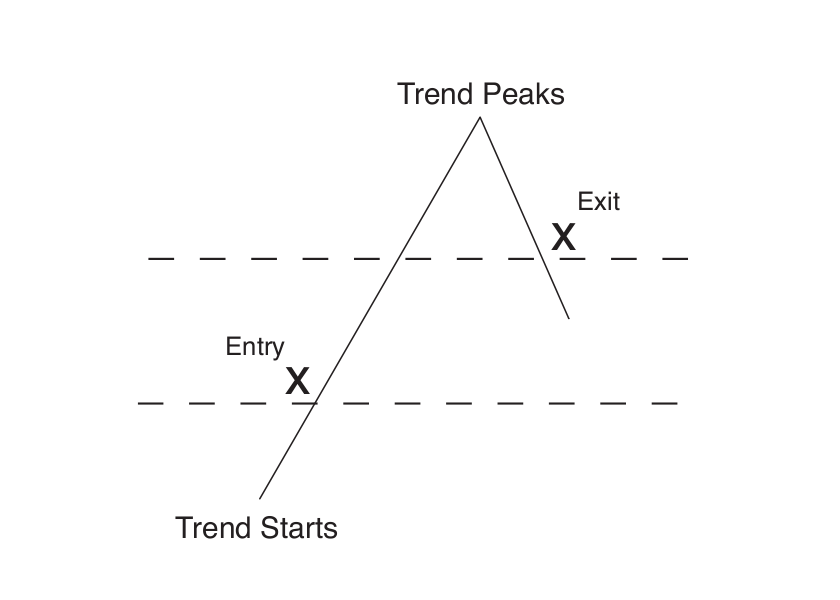
\includegraphics[scale=.2]{trend_following.png}
  \end{center}
  \caption{Simple example of how trend following works in practise (\cite{Trend01})}
\end{figure}

Another advantage of this investing method is the fact that investor does not have to know much about what is being traded (it could be stocks, oil, gold, etc.).
Normally, people tend to gather some information about the company they are willing to invest in. 
They analyse its market situation, competitors, financial performance, etc. which is time consuming, especially for someone who is not a professional trader.
With trend following we just have to focus on elaborating trading rules that should reflect our trading strategy.
After that, we can automate the decision making process by designing and implementing our own trading system.   

\subsection{Types of trends}
\label{sec:types_of_trends}

There are three main types of trends:

\begin{enumerate}
  \item \textbf{Short-term trend}: any price movement that occurs over a few hours or days.
  \item \textbf{Intermediate-term trend}: general movement in price data that lasts from three weeks to six months.
  \item \textbf{Long-term trend}: any price movement that occurs over a significant period of time, often over one year or several years.
\end{enumerate}



\subsection{Designing trading system based on trend following} 

Following \cite{Trend01}, the core of each trading system based on trend following strategy is a set of rules governing each buy/sell decision.
More specifically we have to devise rules to answer the following questions:

\begin{itemize}
  \item how much money are we willing to put on a single trade;
  \item when to exit (what kind of losses are acceptable);
  \item when to enter (when the trend has started); 
  \item what markets are we interested in and how to split money between them (we would like to have a diverse portfolio (stocks, gold, etc.)).
\end{itemize}

These rules should reflect our investing style.

Simple Moving Average (SMA) is especially useful to highlight longer-term trends in a set of data points \cite{Trend01}.

SMA is formulated as the unweighted mean of the previous $N$ data points \cite{Trend01}:

\begin{equation}
    SMA_{today,N} = \frac{\sum_{i=1}^{N}p_{today - i}}{N}
\end{equation}

\begin{description}
  \item [$p_{j}$] 
    value of data on day $j$
\end{description}

In this case, data points will represent closing stock prices. 
 


\textbf{Entry points:}
  \begin{itemize}
    \item Simple moving average (SMA) of last $N$ days is greater than SMA of last $M$ days ($N$ < $M$);
    \item Current stock price is max of last $N$ days (that is usually a good indicator of lucrative opportunity on the market).
  \end{itemize}

As soon as at least one of the above conditions is satisfied we go long (we buy a particular asset).


\textbf{Exit points:}
  \begin{itemize}
    \item Losses on a single trade are greater than 2 \% (this rule is used to quickly abandon an investment that we were wrong about its trend direction,
	  the amount of tolerable loss solely depends on our strategy and does not have to be exactly 2\%);
    \item Simple moving average (SMA) of last $N$ days is lesser than SMA of last $M$ days ($N$ < $M$).
  \end{itemize}

As soon as the exit condition is satisfied we go short (we sell a particular asset).
 
Obviously the above rules are very simple and quite straightforward.
Nonetheless, the system based on them proves to be robust, as shown in chapter \ref{sec:experiments}.
   
By manipulating the value of $N$ we can seek out different types of trends, as mentioned in \ref{sec:types_of_trends}. 

\subsection{Pseudocode}

Algorithm~\ref{fig:tf_pseudo} shows pseudocode of trend following. It uses the following functions:


\begin{description}

\item[SMA(i,N)]
  calculates Simple Moving Average for stock $i$, $N$ last days are taken into account  
\item[go\_short(i)]
  sell stock $i$
\item[go\_long(i)]
  buy stock $i$
\item[get\_current\_stock\_price(i, day)]
  returns stock $i$ price for specific $day$ 
\item[get\_most\_recent\_trade\_price(i)]
  returns the price we paid for stock $i$ (we have stock $i$ in our portfolio)
\item[max(i,N)]
  returns the maximum price for stock $i$ in the last $N$ days
\item[N, M, maximal\_value\_loss]
  modifiable parameters
\end{description}
% 


% \begin{algorithmic}
% 
% \STATE $maximal\_value\_loss \gets 0.98$
% 
% \FOR{$day = 1$ to $max\_day$} 
% 
%   \FOR{$i = 1$ to $number\_of\_stocks$}
% 
%     \IF {$ get\_most\_recent\_trade\_price(i) < maximal\_value\_loss * get\_current\_stock\_price(i, day) $} 
% 	    \STATE $go\_short(i)$
%     \ELSE
% 	    \IF {$SMA(i,N) < SMA(i,M)$}
% 		    \STATE $go\_short(i)$
% 	    \ENDIF
%     \ENDIF
% 
%     \IF {$SMA(i,N) > SMA(i,M)$} 
% 	    \STATE $go\_long(i)$
%     \ELSE
% 	    \IF {$max(i,N)) <= get\_current\_stock\_price(i, day)$}
% 		    \STATE $go\_long(i)$
% 	    \ENDIF
%     \ENDIF
% 
%   \ENDFOR
% 
% \ENDFOR
% 
% \end{algorithmic}

\begin{algorithm}
  \SetKwData{parents}{parents}
  \SetKwData{maxDays}{maxDays}
  \SetKwData{numberOfStocks}{numberOfStocks}
  \SetKwData{maximumValueLoss}{maximumValueLoss}
 
  \SetKwFunction{SMA}{SMA}
  \SetKwFunction{getMaxStockPrice}{getMaxStockPrice}
  \SetKwFunction{goShort}{goShort}
  \SetKwFunction{goLong}{goLong}
  \SetKwFunction{getMostRecentTradePrice}{getMostRecentTradePrice}
  \SetKwFunction{getCurrentStockPrice}{getCurrentStockPrice}
  \SetKwFunction{mutateLeastFitIndividuals}{mutateLeastFitIndividuals}
  \SetKwFunction{extinctLeastFitIndividuals}{extinctLeastFitIndividuals}
  \SetKwInOut{Input}{input}\SetKwInOut{Output}{output}
 
  \Input{$N$, $M$}
  \BlankLine
  \maximumValueLoss $\leftarrow$ 0.98 \;
  
  \For{$day\leftarrow 1$ \KwTo \maxDays}{

     \For{$i\leftarrow 1$ \KwTo \numberOfStocks}{
      
      \BlankLine

	\If(){\getMostRecentTradePrice{$i$} < \maximumValueLoss * \getCurrentStockPrice{$i$, $day$} }{
	  \goShort{$i$} \;
      }
      \ElseIf{\SMA{$i$, $N$} < \SMA{$i$, $M$}}{
	   \goShort{$i$} \;
	}

      \BlankLine

      \If(){\SMA{$i$, $N$} > \SMA{$i$, $M$} }{
	  \goLong{$i$} \;
      }
      \ElseIf{\getMaxStockPrice{$i$, $N$} <= \getCurrentStockPrice{$i$, $day$} }{
	   \goLong{$i$} \;
	}


    }
  }
  \caption{Trend following pseudocode}\label{fig:tf_pseudo}
\end{algorithm}
